\documentclass[fr]{../../../eplsummary}

\usepackage{../../../eplunits}
\usepackage{../../../eplelec}
\usepackage{circuitikz}
\sisetup{detect-all}

\newcommand{\Ueff}{U_\text{eff}}
\newcommand{\Ieff}{I_\text{eff}}
\newcommand{\Umr}{U_\text{moy,r}}
\newcommand{\Imr}{I_\text{moy,r}}

\makeatletter
\providecommand\add@text{}
\renewcommand\u[1]{%
  \gdef\add@text{[\si{#1}\gdef\add@text{}]}}% 
\renewcommand\tagform@[1]{%
  \maketag@@@{\llap{\add@text\quad}(\ignorespaces#1\unskip\@@italiccorr)}%
}

\hypertitle{Convertisseurs électromécaniques}{6}{ELEC}{1310}
{Antoine Paris}
{Bruno Dehez}

\part{Rappels des notions de bases}
Avant tout, rappelons les notations utilisées dans le cours.
\begin{itemize}
	\item Les lettres minuscules $i$ et $u$ décrivent
	la valeur instantanée du courant et de la tension ;
	\item $U_c$, $U_p$ ou $U_\text{max}$ (idem avec $I$)
	donne la valeur de crête (\emph{peak}) de la tension
	(ou de courant) ;
	\item $U$ ou $\Ueff$ (idem avec $I$) donne la
	valeur efficace (ou RMS) de la tension ;
	\item $\Umr$ et $\Imr$ donnent
	la valeur moyenne redressée de la tension et du courant ;
	\item $ff_u$ et $ff_i$ donnent le facteur de forme de
	la tension et du courant. 
\end{itemize}

\section{Définitions}
\begin{mynota}
On note $<g>$ la moyenne d'une fonction quelconque du temps
$g$.
\end{mynota}

\begin{mydef}[Valeur efficace]
\begin{align}
	U = \Ueff & \eqdef \sqrt{<u^2>} & I = \Ieff & \eqdef \sqrt{<i^2>}. 
\end{align}
Dans le cadre de ce cours, et si ce n'est pas précisé, on suppose
toujours que les valeurs données sont des valeurs efficaces.
\end{mydef}

\begin{mydef}[Moyenne redressée]
\begin{align}
	\Umr & \eqdef <|u|> & \Imr & \eqdef <|i|>. 
\end{align}
\end{mydef}

\begin{mydef}[Facteur de forme]
\begin{align}
	ff_u & \eqdef \frac{U}{\Umr} & ff_i & \eqdef \frac{I}{\Imr}. 
\end{align}
\end{mydef}

\subsection{Cas particulier d'une grandeur périodique}
Soit une grandeur $g$. Cette grandeur est \textbf{périodique} si
\[ \exists T \text{ tel que } \forall t \Rightarrow g(t+T)= g(t). \]
On définit alors
\begin{align*}
	f & \eqdef \frac{1}{T} & \omega & \eqdef 2\pi f.
\end{align*}

Dans ce cas particulier, la valeur moyenne devient
\begin{equation}
	<g> = \frac{1}{T} \int_0^T g \dif t
\end{equation}
et la valeur efficace devient
\begin{equation}
	G = \sqrt{<g^2>} = \sqrt{\frac{1}{T} \int_0^T g^2 \dif t}.
\end{equation}

\begin{mydef}[Grandeur alternative]
Une grandeur \textbf{alternative} est une grandeur périodique
de valeur moyenne nulle.
\end{mydef}

\subsection{Cas particulier d'une grandeur sinusoïdale}
Si $g$ est une grandeur sinusoïdale, on peut l'écrire de façon
tout à fait générale
\[ g = G_c \cos(\omega t + \varphi_g). \]
En terme de courant et de tension, cela donne
\begin{align}
	u & = U_c \cos(\omega t + \varphi_u) & i & = I_c \cos(\omega t + \varphi_i).
	\label{eq:sin-form-peak}
\end{align}
Dans ce cas particulier \textbf{uniquement}, on a démonté au cours
de physique 1 que
\begin{align}
	U_c & = \sqrt{2}U & I_c & = \sqrt{2}I.
\end{align}
On peut dont réecrire l'équation \ref{eq:sin-form-peak}
\begin{align}
	u & = \sqrt{2}U \cos(\omega t + \varphi_u) & i & = \sqrt{2}I \cos(\omega t + \varphi_i).
\end{align}
On préfère en général cette dernière forme car elle utilise les
valeurs efficaces de courant et tension.

\begin{mydef}[Déphasage]
On définit le déphasage $\varphi$ entre la tension et le courant
\begin{equation}
	\varphi \eqdef \varphi_u - \varphi_i.
\end{equation}
Si $\varphi > 0$, on dit que la tension est en avance sur le courant.
Dans le cas contraire, on dit que la tension est en retard sur le
courant.
\end{mydef}

\section{Phaseurs}
\subsection{Généralités}
\`{A} chaque grandeur sinusoïdale $g = \sqrt{2}G \cos(\omega t
+ \varphi_g)$, on peut associer un \textbf{phaseur}
\begin{equation}
	\bar{G} = Ge^{j\varphi_g}.
\end{equation}

\begin{myrem}
Le module du phaseur est égal à la \textbf{valeur efficace} de
la grandeur sinusoïdale.
\end{myrem}

On peut bien sur réecrire ce phaseur en faisant apparaître
une partie réelle et une partie imaginaire et le réprésenter
sur un diagramme phasoriel comme illustré à la figure
\ref{fig:dia-phasoriel}.

\begin{figure}[ht]
	\centering
	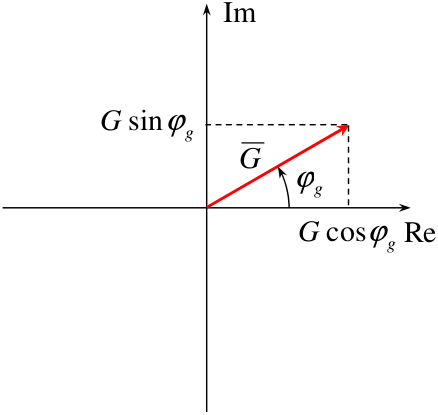
\includegraphics[scale=0.35]{img/dia-phasoriel.png}
	\caption{Diagramme phasoriel.}
	\label{fig:dia-phasoriel}
\end{figure}

On peut retrouver l'expression temporelle d'une grandeur
sinusoïdale en multipliant son phaseur par $e^{j\omega t}$
et en prenant la partie réelle
\begin{equation}
	\Re(\bar{G}e^{j\omega t}) = G\cos(\omega t + \varphi_g) =
	\frac{g}{\sqrt{2}}.
\end{equation}

\subsection{Opérations sur les phaseurs}
On est souvent amené à effectuer des opérations sur les phaseurs,
comme des sommes (en appliquant KCL ou KVL), des
multiplication (pour des calculs de puissances) ou des dérivées
et des intégrales (avec une inductance ou une capacitance).

Lorsqu'on effectue ces opérations il ne faut bien sur pas oublier
qu'un phaseur est un complexe et dont peut être représenté comme
un vecteur.

\paragraph{Addition}
\begin{align*}
	\bar{G}_\text{tot} 	& = \bar{G}_1 + \bar{G}_2 \\
						&= (G_1\cos \varphi_{g1} + G_2\cos \varphi_{g2})
						+ j(G_1\sin \varphi_{g1} + G_2\cos \varphi_{g2})
\end{align*}

\paragraph{Multiplication}
\begin{align*}
	\bar{G}_\text{tot} 	& = \bar{G}_1 \cdot \bar{G}_2 \\
						&= G_1G_2 e^{j(\varphi_{g1} + \varphi_{g2})}
\end{align*}

\paragraph{Dérivation}
\begin{equation*}
	\fdif{\bar{G}}{t} = j\omega\bar{G} = e^{j\frac{\pi}{2}}\omega
	\bar{G} = \omega G e^{j(\varphi + \frac{\pi}{2})}
\end{equation*}

Pour une inductance dont la relation courant-tension est donnée par
$v = L\fdif{i}{t}$, on retrouve bien que la tension est en avance
de 90° sur le courant.

\paragraph{Intégration}
\begin{equation*}
	\int \bar{G} \dif t = \frac{\bar{G}}{j\omega}
	= e^{-j\frac{\pi}{2}}\frac{\bar{G}}{j\omega}
	= \frac{G}{\omega}e^{j(\varphi-\frac{\pi}{2})}
\end{equation*}

Pour une capacitance dont la relation courant-tension est donnée par
$i = c\fdif{v}{t}$, on retrouve bien que la tension est en retard
de 90° sur le courant.

% TODO: convention récepteur/émetteur

\section{Puissances}
Dans cette section, on définit les différentes puissance dans le cas
particulier de tension et courant sinusoïdals.

\begin{mydef}[Puissance instantanée]
La puissance instantanée $p$ d'un élément de circuit
est donnée par
\begin{equation}
	p \eqdef ui \stackrel{sin}{=} <p> + UI\cos(2\omega t +
	\varphi_u + \varphi_i)
	\u{\watt}
\end{equation}
où $u$ est la tension instantanée aux bornes de cet élément
et $i$ le courant le traversant. On remarque donc que la
puissance instantannée est constituée d'une partie constante
égale à la puissance moyenne et d'une partie oscillante à 2 fois
la fréquence de la tension et du courant.
\end{mydef}

\begin{mydef}[Puissance complexe]
La puissance complexe $\bar{S}$ d'un élément est donnée par
\begin{equation}
	\bar{S} \eqdef \frac{1}{2}\bar{V}\bar{I}^*
	\stackrel{sin}{=} UIe^{j\varphi}. 
	\u{\volt\ampere}
\end{equation}
On peut décomposer cette puissance complexe en une partie
réelle $P$ qu'on appelle la puissance active et une partie
imaginaire $Q$ qu'on appelle la puissance réactive.
\begin{equation}
	\bar{S} = P + jQ.
\end{equation}
La norme $S$ de $\bar{S}$ est appelée la puissance apparente.
\end{mydef}

\begin{mydef}[Puissance active]
La puissance \textbf{active} $P$ est la moyenne de la
puissance instantanée
\begin{equation}
	P \eqdef\Re(\bar{S}) \stackrel{sin}{=} <p> = <ui>
	= UI\cos(\varphi).
	\u{\watt}
\end{equation}
Par défaut, lorsqu'on parle de puissance d'une impédance, on
parle de puissance active. Intuitivement, la puissance active
traduit un échange d'énergie unilatéral entre la source et
une charge. En d'autres termes, il s'agit de la puissance
dissipée et perdue à tout jamais (dans une résistance par exemple).
Dans cette dernière équation, on remarque que $P = 0$ si $\varphi =
\pm \frac{\pi}{2}$. C'est à dire si l'élément est purement inductif
ou capacitif. 
\end{mydef}

\begin{mydef}[Puissance réactive]
La puissance \textbf{réactive} $Q$ n'apparaît qu'en présence
d'un élément inductif ou capacitif. Elle traduit un échange bilatéral
d'énergie entre la source et la charge. En d'autres termes, il
s'agit de la puissance stockée et reçue de manière réversible dans
l'impédance.
\begin{equation}
	Q \eqdef \Im(\bar{S}) \stackrel{sin}{=} UI\sin(\varphi).
	\u{\volt\ampere r}
\end{equation}
Ses unités sont des volts ampères réactifs.
On remarque bien dans cette dernière équation que $Q = 0$ si
$\varphi = 0$, c'est à dire si le courant et la tension sont
parfaitement en phase et donc que l'élément de circuit est purement
résistif. 

On parle d'éléments inductifs lorsqu'ils \og absorbent \fg{} de
la puissance réactive ($Q > 0$), c'est à dire quand
\[ 0 < \varphi \leq \frac{\pi}{2} \]
et d'éléments réactifs lorsqu'ils \og produisent \fg{} de la
puissance réactive ($Q < 0$), c'est à dire quand
\[ -\frac{\pi}{2} \leq \varphi < 0. \]
\end{mydef}

\begin{mydef}[Puissance apparente]
La puissance \textbf{apparente} $S$ est le  produit des
valeurs efficaces de la tension et du courant
\begin{equation}
	S \eqdef |\bar{S}| = \sqrt{P^2 + Q^2} \stackrel{sin}{=} UI.
	\u{\volt\ampere}
\end{equation}
\end{mydef}

\begin{mydef}[Facteur de puissance]
On définit le facteur de puissance $fp$
\begin{equation}
	fp \eqdef \frac{P}{S} \stackrel{sin}{=} \cos\varphi.
\end{equation}
\end{mydef}

\section{Impédances}
\subsection{Généralités}
\begin{mydef}
En phasoriel, l'impédance se définit
\begin{equation}
	\bar{Z} \eqdef \frac{\bar{U}}{\bar{I}}.
\end{equation}
Son utilisation n'est valable que dans le cas
\begin{itemize}
	\item d'un régime sinusoïdal établi ;
	\item de composants linéraires.
\end{itemize}
\end{mydef}

On retrouve facilement les impédances des éléments
de circuits habituels.
\begin{align*}
	\bar{Z} & = R 					& \text{pour une résistance,} \\
	\bar{Z} & = j\omega L 			& \text{pour une inductance,} \\
	\bar{Z} & = \frac{1}{j\omega C}	& \text{pour une capacitance.} 
\end{align*}
On remarque que l'impédance est une fonction de la fréquence pour
l'inductance et la capacitance.

\begin{myrem}
Quand l'effet de peau n'est pas négligeable (à haute fréquence), la
résistance dépend également de la fréquence (voir cours
LELEC1350 - électromagnétisme appliqué).
\end{myrem}

On simplifie des impédances en séries et en parallèles de la même
manière que des résistances (en gardant en tête que l'impédance est
un nombre comlexe).

\subsection{Substitutions étoile - triangle}
En régime triphasé on est régulièrement amené à travailler avec des
configurations d'impédances en étoile ou en triangle comme illustré à la
figure \ref{fig:sub-star-triangle}.

\begin{figure*}[ht!]
    \centering
    \begin{subfigure}[t]{0.45\textwidth}
        \centering
        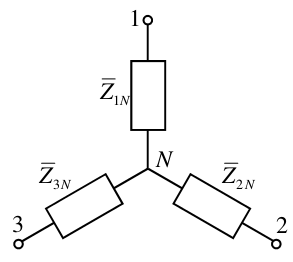
\includegraphics[height=1.2in]{img/star.png}
        \caption{En étoile.}
    \end{subfigure}%
    $\Longrightarrow$
    \begin{subfigure}[t]{0.45\textwidth}
        \centering
        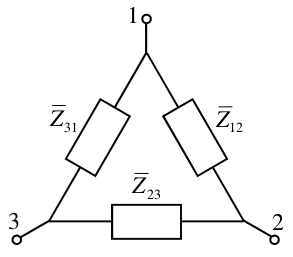
\includegraphics[height=1.2in]{img/triangle.png}
        \caption{En triangle.}
    \end{subfigure}
    \caption{Subsitutions étoile - triangle}
    \label{fig:sub-star-triangle}
\end{figure*}

On peut passer de triangle à étoile en utilisant
\begin{align*}
	\bar{Z}_{1N} &= \frac{\bar{Z}_{31}\bar{Z}_{12}}{\bar{Z}_{12}+\bar{Z}_{23}+\bar{Z}_{31}} &
	\bar{Z}_{2N} &= \frac{\bar{Z}_{12}\bar{Z}_{23}}{\bar{Z}_{12}+\bar{Z}_{23}+\bar{Z}_{31}} &
	\bar{Z}_{3N} &= \frac{\bar{Z}_{23}\bar{Z}_{31}}{\bar{Z}_{12}+\bar{Z}_{23}+\bar{Z}_{31}}
\end{align*}
et d'étoile à triangle en utilisant
\begin{align*}
	\bar{Z}_{31} &= \bar{Z}_{3N} + \bar{Z}_{1N} + \frac{\bar{Z}_{3N}\bar{Z}_{1N}}{\bar{Z_{2N}}} &
	\bar{Z}_{12} &= \bar{Z}_{1N} + \bar{Z}_{2N} + \frac{\bar{Z}_{1N}\bar{Z}_{2N}}{\bar{Z_{3N}}} &
	\bar{Z}_{23} &= \bar{Z}_{2N} + \bar{Z}_{3N} + \frac{\bar{Z}_{2N}\bar{Z}_{3N}}{\bar{Z_{1N}}}.
\end{align*}

Fort heureusement, ces horribles formules se simplifient grandement dans
le cas de configurations équilibrées, c'est à dire quand $\bar{Z}_{1N} =
\bar{Z}_{2N} = \bar{Z}_{3N} = \bar{Z}_N$ et quand $\bar{Z}_{31} = \bar{Z}_{12} =
\bar{Z}_{23} = \bar{Z}$. Dans ce cas, on peut passer de triangle à étoile en utilisant
\begin{equation*}
	\bar{Z}_N = \frac{\bar{Z}}{3}
\end{equation*}
et d'étoile à triangle en utilisant
\begin{equation*}
	\bar{Z} = 3\bar{Z}_N.
\end{equation*}

\section{Mesures en électrotechnique}
\subsection{Généralités}
Les mesures des \textbf{valeurs efficaces} de la tension et du
courant s'effectuent respectivement avec un voltmètre
et un ampèremètre. On peut également mesurer la
\textbf{puissance active} à l'aide d'un wattmètre.

Lorsqu'on effectue des mesures, il faut faire attention
aux erreurs causées par l'insertion d'un appareil de mesure
(voir figure \ref{fig:mes-errors}).

\begin{figure*}[ht!]
    \centering
    \begin{subfigure}[t]{0.5\textwidth}
        \centering
        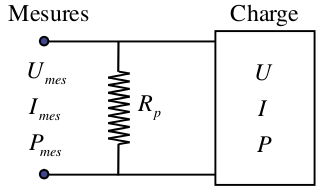
\includegraphics[height=1.2in]{img/mes-insert.png}
        \caption{Dans cet exemple, on souhaite mesurer la tension
        $U$ à l'aide d'un voltmère que l'on connecte donc en parallèle
        avec la charge. La résistance interne du voltmètre $R_p$ est
        donc en parallèle avec la charge et va perturber le
        fonctionnement du circuit. Pour un voltmètre idéal,
        $R_p \to \infty$ et on peut négliger cette perturbation.}
    \end{subfigure}%
    ~
    \begin{subfigure}[t]{0.5\textwidth}
        \centering
        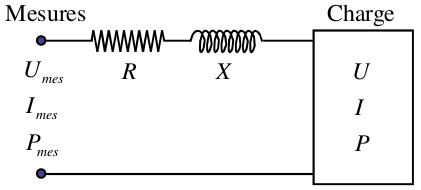
\includegraphics[height=1.2in]{img/mes-bad-link.png}
        \caption{Dans cet exemple, on souhaite mesurer le courant
        $I$ circulant dans la charge à l'aide d'un ampèremètre que l'on
        connecte donc en série avec la charge. L'impédance interne
        du voltmètre, constitué ici d'une résistance $R$ et d'une
        inductance $X$, va perturber le circuit. Pour
        un ampèremètre idéal, $R$ et $X \to 0$ et on peut négligler
        cette pertubation.}
    \end{subfigure}
    \caption{Erreur de mesure due à l'insertion d'un appareil
    de mesure (a) et erreur de mesure due à une liaison non-idéale (b).}
    \label{fig:mes-errors}
\end{figure*}

\subsection{Mesures d'impédances}
Pour mesurer une impédance, c'est à dire un nombre complexe,
il faut effectuer deux mesures
\begin{align*}
	|\bar{Z}| & = Z = \frac{U_\text{mes}}{I_\text{mes}}, \\
	\arg \bar{Z} & = \varphi = \arccos\left(\frac{P_\text{mes}}
	{U_\text{mes}I_\text{mes}}\right).
\end{align*}
% FIX: discussion avec @cassiersg, @bilal1509 et @pverbist sur la formule
% pour l'argument de Z.

On peut ensuite trouver un circuit équivalent série (figure
\ref{fig:eq-circ} (a))
\begin{align*}
	R_s & = Z\cos\varphi & X_s & = \sin\varphi
\end{align*}
et un circuit équivalent parallèle (figure \ref{fig:eq-circ} (b))
\begin{align*}
	R_p & = \frac{Z}{\cos\varphi} & X_p & = \frac{Z}{\sin\varphi}.
\end{align*}

\begin{figure*}[ht!]
    \centering
    \begin{subfigure}[t]{0.5\textwidth}
        \centering
        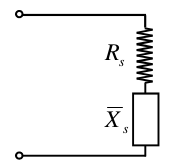
\includegraphics[height=1.2in]{img/eq-circ-series.png}
        \caption{Circuit équivalent série.}
    \end{subfigure}%
    ~
    \begin{subfigure}[t]{0.5\textwidth}
        \centering
        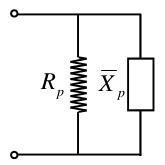
\includegraphics[height=1.2in]{img/eq-circ-para.png}
        \caption{Circuit équivalent parallèle.}
    \end{subfigure}
    \caption{Circuits équivalents d'une impédance.}
    \label{fig:eq-circ}
\end{figure*}

\part{Les transformateurs de puissance}

\part{Les convertisseurs électromécaniques}

\end{document}
